\documentclass[border=10pt]{standalone}
\usepackage{tikz}
\usetikzlibrary{shapes, positioning, arrows.meta, calc}

\begin{document}
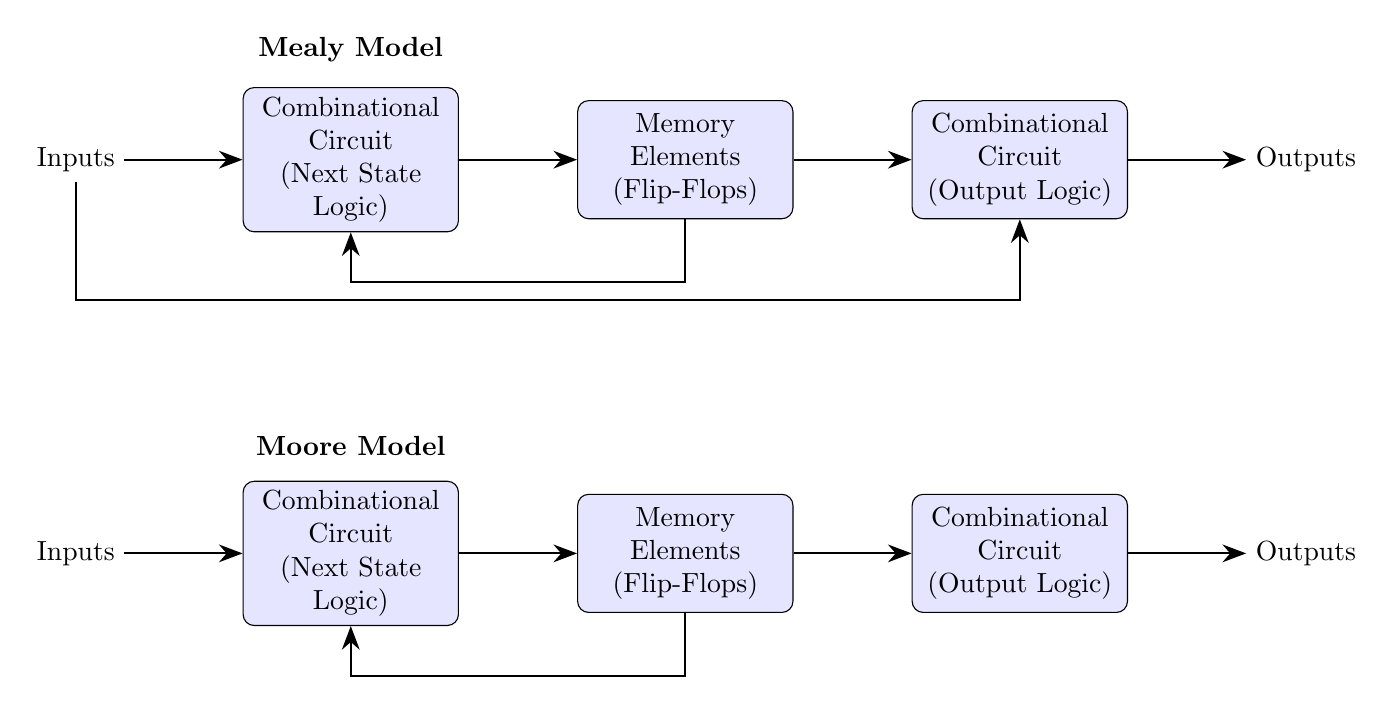
\begin{tikzpicture}[
    auto,
    block/.style={rectangle, draw, fill=blue!10, text width=2.5cm, text centered, rounded corners, minimum height=1.5cm},
    line/.style={draw, -{Stealth[length=3mm]}, thick},
    node distance=1.5cm
]

    %% MEALY MODEL
    \begin{scope}
        \node (input) {Inputs};
        \node [block, right=of input] (nextstate) {Combinational\\Circuit\\(Next State Logic)};
        \node [block, right=of nextstate] (memory) {Memory\\Elements\\(Flip-Flops)};
        \node [block, right=of memory] (outputlog) {Combinational\\Circuit\\(Output Logic)};
        \node [right=of outputlog] (output) {Outputs};

        % Paths
        \path [line] (input) -- (nextstate);
        \path [line] (nextstate) -- (memory);
        \path [line] (memory) -- (outputlog);
        \path [line] (outputlog) -- (output);
        
        % Feedback
        \draw [line] (memory.south) -- ++(0,-0.8) -| (nextstate.south);
        
        % Mealy Feature: Input directly to Output Logic
        \draw [line] (input.south) -- ++(0,-1.5) -| (outputlog.south);
        
        \node [above=0.2cm of nextstate, font=\bfseries] {Mealy Model};
    \end{scope}

    %% MOORE MODEL - Positioned below Mealy
    \begin{scope}[yshift=-5cm]
        \node (minput) {Inputs};
        \node [block, right=of minput] (mnextstate) {Combinational\\Circuit\\(Next State Logic)};
        \node [block, right=of mnextstate] (mmemory) {Memory\\Elements\\(Flip-Flops)};
        \node [block, right=of mmemory] (moutputlog) {Combinational\\Circuit\\(Output Logic)};
        \node [right=of moutputlog] (moutput) {Outputs};

        % Paths
        \path [line] (minput) -- (mnextstate);
        \path [line] (mnextstate) -- (mmemory);
        \path [line] (mmemory) -- (moutputlog);
        \path [line] (moutputlog) -- (moutput);
        
        % Feedback
        \draw [line] (mmemory.south) -- ++(0,-0.8) -| (mnextstate.south);
        
        % Moore Feature: Output depends ONLY on Memory (No direct input path to output logic)
        % (So we just leave it as is)
        
        \node [above=0.2cm of mnextstate, font=\bfseries] {Moore Model};
    \end{scope}

\end{tikzpicture}
\end{document}
